\documentclass[a4paper,11pt]{article}
\usepackage[utf8]{inputenc}
\usepackage[T1]{fontenc}
\usepackage[english]{babel}
\usepackage{lmodern}\usepackage{microtype}
\usepackage{amsmath,amssymb,bm,mathtools}
\usepackage{geometry}
\geometry{a4paper,left=2.3cm,right=2.3cm,top=2.0cm,bottom=2.0cm}
\usepackage{booktabs,array}
\usepackage{xcolor}\definecolor{bokug}{RGB}{0,135,60}
\usepackage{tikz}
\usetikzlibrary{patterns,arrows.meta,calc,decorations.pathmorphing}
\usepackage{fancyhdr}\pagestyle{fancy}
\renewcommand{\headrulewidth}{0.4pt}
\usepackage{enumitem}\setlength{\parindent}{0pt}\setlength{\parskip}{4pt}

\begin{document}
\fancyhead[L]{\small VU Mechanik – LAWI 100515 (PI)}
\fancyhead[R]{\small SS 2026}
\fancyfoot[C]{\thepage}
\begin{center}{\large\bfseries\color{bokug}University of Natural Resources and Life Sciences, Vienna (BOKU)}\\[2pt]{\large\bfseries VU Mechanik – LAWI 100515 (PI)}\\[4pt]Exam \textbf{Group A} \hfill Date: 26.06.2026\\[2pt]\rule{\linewidth}{0.4pt}\end{center}

\begin{center}\textbf{\large Model solution}\end{center}
\begin{center}
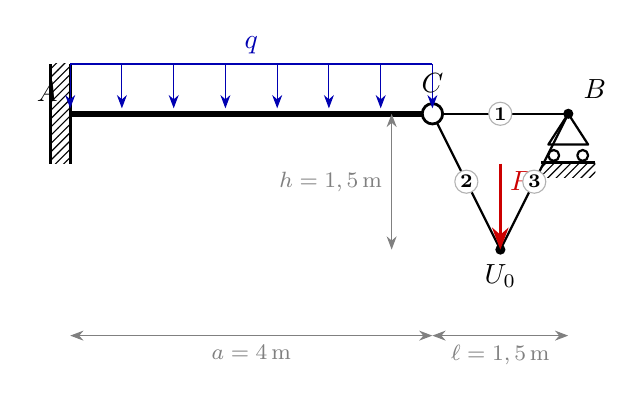
\begin{tikzpicture}[scale=1.15, rotate=0, >=Stealth, line join=round]
  \coordinate (A) at (0.000,0.000);
  \coordinate (C) at (4.000,0.000);
  \coordinate (O1) at (5.500,0.000);
  \coordinate (U0) at (4.750,-1.500);
  \draw[thick] (C) -- (O1);
  \draw[thick] (C) -- (U0);
  \draw[thick] (U0) -- (O1);
  \draw[line width=2.2pt] (A) -- (C);
  \fill (C) circle (1.6pt);
  \fill (O1) circle (1.6pt);
  \fill (U0) circle (1.6pt);
  \draw[fill=white,line width=1pt] (C) circle (3.2pt);
  \draw[line width=1.1pt] (0.000,-0.550) -- (0.000,0.550);
  \fill[pattern=north east lines] (-0.220,-0.550) rectangle (0.000,0.550);
  \draw[line width=1.1pt] (-0.220,-0.550) -- (-0.220,0.550);
  \draw[thick] (5.500,0.000) -- (5.280,-0.340) -- (5.720,-0.340) -- cycle;
  \draw[thick] (5.340,-0.460) circle (0.06) (5.660,-0.460) circle (0.06);
  \draw[line width=1.1pt] (5.200,-0.540) -- (5.800,-0.540);
  \fill[pattern=north east lines] (5.200,-0.700) rectangle (5.800,-0.540);
  \draw[blue!70!black,thick] (0.000,0.550) -- (4.000,0.550);
  \draw[->,blue!70!black] (0.000,0.550) -- (0.000,0.06);
  \draw[->,blue!70!black] (0.571,0.550) -- (0.571,0.06);
  \draw[->,blue!70!black] (1.143,0.550) -- (1.143,0.06);
  \draw[->,blue!70!black] (1.714,0.550) -- (1.714,0.06);
  \draw[->,blue!70!black] (2.286,0.550) -- (2.286,0.06);
  \draw[->,blue!70!black] (2.857,0.550) -- (2.857,0.06);
  \draw[->,blue!70!black] (3.429,0.550) -- (3.429,0.06);
  \draw[->,blue!70!black] (4.000,0.550) -- (4.000,0.06);
  \node[blue!70!black,above] at (2.000,0.550) {$q$};
  \draw[->,red!80!black,line width=1.1pt] (4.750,-0.550) -- (4.750,-1.500);
  \node[red!80!black,above right] at (4.750,-0.950) {$P$};
  \node[circle,fill=white,draw=gray!60,inner sep=0.7pt,font=\scriptsize] at (4.750,0.000) {\textbf{1}};
  \node[circle,fill=white,draw=gray!60,inner sep=0.7pt,font=\scriptsize] at (4.375,-0.750) {\textbf{2}};
  \node[circle,fill=white,draw=gray!60,inner sep=0.7pt,font=\scriptsize] at (5.125,-0.750) {\textbf{3}};
  \node[above left=1pt] at (A) {$A$};
  \node[above=4pt] at (C) {$C$};
  \node[above right=2pt] at (O1) {$B$};
  \node[below=2pt] at (U0) {$U_{0}$};
  \draw[<->,gray] (0.000,-2.450) -- (4.000,-2.450) node[midway,below,font=\footnotesize]{$a=4$\,m};
  \draw[<->,gray] (4.000,-2.450) -- (5.500,-2.450) node[midway,below,font=\footnotesize]{$\ell=1,5$\,m};
  \draw[<->,gray] (3.550,0) -- (3.550,-1.500) node[midway,left,font=\footnotesize]{$h=1,5$\,m};
\end{tikzpicture}
\end{center}
\par\medskip\textbf{1.\ Static determinacy}\\[-2pt]
Counting criterion $n = r - (3 + v)$ with $r$ support reactions and $v$ hinge conditions:
\[ n = r - (3+v) = 4 - (3+1) = 0 \quad\Rightarrow\quad \text{the system is statically determinate.} \]
\par\medskip\textbf{2.\ Support reactions and hinge force}\\[-2pt]
$A_x = 0$\,kN,\quad $A_y = 30$\,kN,\quad $M_A = 80$\,kNm,\quad $B_x = 0$\,kN,\quad $B_y = 10$\,kN\\[2pt]$C_x = 0$\,kN,\quad $C_y = -10$\,kN\par
\par\medskip\textbf{3.\ Truss member forces}\par
\begin{center}\renewcommand{\arraystretch}{1.15}
\begin{tabular}{c r l}
\toprule
Member & Member force $S$ [kN] & Type \\
\midrule
  1 (C\,--\,O1) & -5 & compression \\
  2 (C\,--\,U0) & 11.18 & tension \\
  3 (U0\,--\,O1) & 11.18 & tension \\
\bottomrule
\end{tabular}\end{center}
\begin{center}
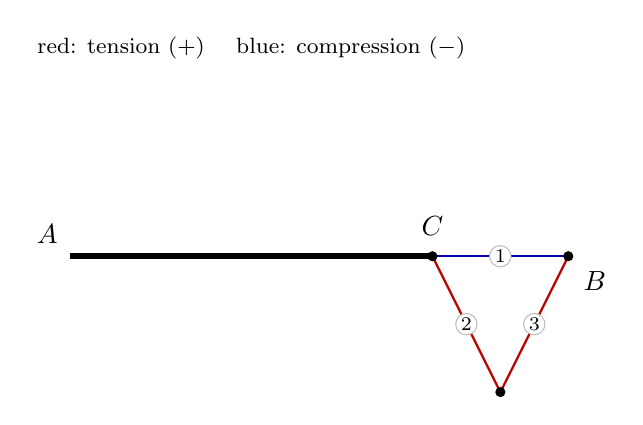
\begin{tikzpicture}[scale=1.15, rotate=0, >=Stealth, line join=round]
  \coordinate (A) at (0.000,0.000);
  \coordinate (C) at (4.000,0.000);
  \coordinate (O1) at (5.500,0.000);
  \coordinate (U0) at (4.750,-1.500);
  \draw[thick,blue!70!black] (C) -- (O1);
  \draw[thick,red!75!black] (C) -- (U0);
  \draw[thick,red!75!black] (U0) -- (O1);
  \draw[line width=2.2pt] (A) -- (C);
  \fill (C) circle (1.6pt);
  \fill (O1) circle (1.6pt);
  \fill (U0) circle (1.6pt);
  \node[circle,fill=white,draw=gray!50,inner sep=0.6pt,font=\scriptsize] at (4.750,0.000) {1};
  \node[circle,fill=white,draw=gray!50,inner sep=0.6pt,font=\scriptsize] at (4.375,-0.750) {2};
  \node[circle,fill=white,draw=gray!50,inner sep=0.6pt,font=\scriptsize] at (5.125,-0.750) {3};
  \node[above left=1pt] at (A) {$A$};
  \node[above=4pt] at (C) {$C$};
  \node[below right=2pt] at (O1) {$B$};
  \node[font=\footnotesize,align=center] at (2.00,2.30) {red: tension $(+)$ \quad blue: compression $(-)$};
\end{tikzpicture}
\end{center}
\par\medskip\textbf{4.\ Section-force diagrams of the bending beam $A$--$C$}\par
\begin{center}
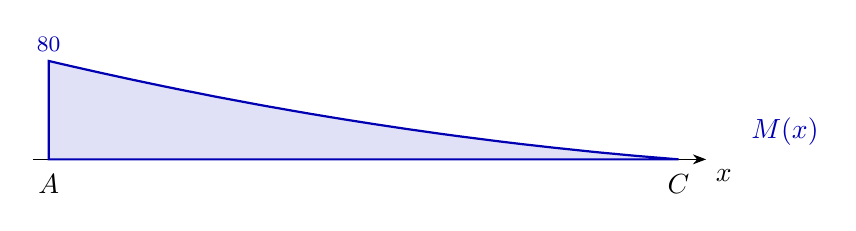
\begin{tikzpicture}[>=Stealth]
  \draw[->] (-0.2,0) -- (8.35,0) node[below right]{$x$};
  \node[below=2pt] at (0,0) {$A$};
  \node[below=2pt] at (8.00,0) {$C$};
  \filldraw[fill=blue!70!black!12,draw=blue!70!black,thick] (0,0) -- plot coordinates {(0.000,1.250) (0.133,1.219) (0.267,1.188) (0.400,1.158) (0.533,1.128) (0.667,1.098) (0.800,1.069) (0.933,1.040) (1.067,1.011) (1.200,0.983) (1.333,0.955) (1.467,0.927) (1.600,0.900) (1.733,0.873) (1.867,0.847) (2.000,0.820) (2.133,0.794) (2.267,0.769) (2.400,0.744) (2.533,0.719) (2.667,0.694) (2.800,0.670) (2.933,0.647) (3.067,0.623) (3.200,0.600) (3.333,0.577) (3.467,0.555) (3.600,0.533) (3.733,0.511) (3.867,0.490) (4.000,0.469) (4.133,0.448) (4.267,0.428) (4.400,0.408) (4.533,0.388) (4.667,0.369) (4.800,0.350) (4.933,0.331) (5.067,0.313) (5.200,0.295) (5.333,0.278) (5.467,0.261) (5.600,0.244) (5.733,0.227) (5.867,0.211) (6.000,0.195) (6.133,0.180) (6.267,0.165) (6.400,0.150) (6.533,0.136) (6.667,0.122) (6.800,0.108) (6.933,0.094) (7.067,0.081) (7.200,0.069) (7.333,0.056) (7.467,0.044) (7.600,0.033) (7.733,0.022) (7.867,0.011) (8.000,-0.000)} -- (8.000,0) -- cycle;
  \node[above,blue!70!black,font=\footnotesize] at (0.000,1.250) {80};
  \node[blue!70!black,right] at (8.80,0.35) {$M(x)$};
\end{tikzpicture}
\\[6pt]
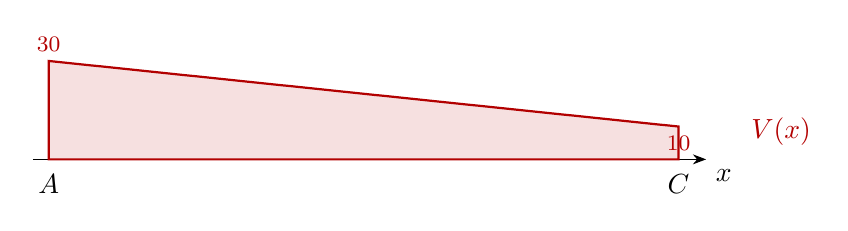
\begin{tikzpicture}[>=Stealth]
  \draw[->] (-0.2,0) -- (8.35,0) node[below right]{$x$};
  \node[below=2pt] at (0,0) {$A$};
  \node[below=2pt] at (8.00,0) {$C$};
  \filldraw[fill=red!70!black!12,draw=red!70!black,thick] (0,0) -- plot coordinates {(0.000,1.250) (0.133,1.236) (0.267,1.222) (0.400,1.208) (0.533,1.194) (0.667,1.181) (0.800,1.167) (0.933,1.153) (1.067,1.139) (1.200,1.125) (1.333,1.111) (1.467,1.097) (1.600,1.083) (1.733,1.069) (1.867,1.056) (2.000,1.042) (2.133,1.028) (2.267,1.014) (2.400,1.000) (2.533,0.986) (2.667,0.972) (2.800,0.958) (2.933,0.944) (3.067,0.931) (3.200,0.917) (3.333,0.903) (3.467,0.889) (3.600,0.875) (3.733,0.861) (3.867,0.847) (4.000,0.833) (4.133,0.819) (4.267,0.806) (4.400,0.792) (4.533,0.778) (4.667,0.764) (4.800,0.750) (4.933,0.736) (5.067,0.722) (5.200,0.708) (5.333,0.694) (5.467,0.681) (5.600,0.667) (5.733,0.653) (5.867,0.639) (6.000,0.625) (6.133,0.611) (6.267,0.597) (6.400,0.583) (6.533,0.569) (6.667,0.556) (6.800,0.542) (6.933,0.528) (7.067,0.514) (7.200,0.500) (7.333,0.486) (7.467,0.472) (7.600,0.458) (7.733,0.444) (7.867,0.431) (8.000,0.417)} -- (8.000,0) -- cycle;
  \node[above,red!70!black,font=\footnotesize] at (0.000,1.250) {30};
  \node[below,red!70!black,font=\footnotesize] at (8.000,0.417) {10};
  \node[red!70!black,right] at (8.80,0.35) {$V(x)$};
\end{tikzpicture}
\\[6pt]
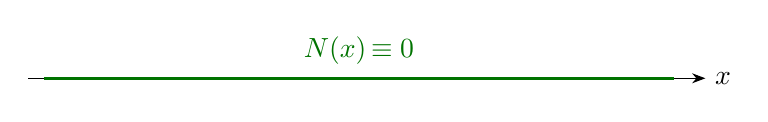
\begin{tikzpicture}[>=Stealth]
  \draw[->] (-0.2,0) -- (8.40,0) node[right]{$x$};
  \draw[green!45!black,very thick] (0,0) -- (8,0);
  \node[green!45!black] at (4,0.35) {$N(x)$\,$\equiv 0$};
\end{tikzpicture}
\end{center}
\end{document}